\documentclass[10pt,xcolor={usenames},fleqn,mathserif,serif]{beamer}

%% colors
\definecolor{bittersweet}{rgb}{1.0, 0.44, 0.37}
\definecolor{brilliantlavender}{rgb}{0.96, 0.73, 1.0}
\definecolor{antiquefuchsia}{rgb}{0.57, 0.36, 0.51}
\definecolor{violetw}{rgb}{0.93, 0.51, 0.93}
\definecolor{Veronica}{rgb}{0.63, 0.36, 0.94}
\definecolor{atomictangerine}{rgb}{1.0, 0.6, 0.4}
\definecolor{darkgray}{rgb}{0.66, 0.66, 0.66}
\definecolor{brightcerulean}{rgb}{0.11, 0.67, 0.84}
\definecolor{cadmiumorange}{rgb}{0.93, 0.53, 0.18}
\definecolor{ochre}{rgb}{0.8, 0.47, 0.13}
\definecolor{midnightblue}{rgb}{0.1, 0.1, 0.44}
\definecolor{lemon}{rgb}{1.0, 0.97, 0.0}
\definecolor{grey}{rgb}{0.7, 0.75, 0.71}
\definecolor{amber}{rgb}{1.0, 0.75, 0.0}
\definecolor{almond}{rgb}{0.94, 0.87, 0.8}
\definecolor{bf}{RGB}{88, 86, 88}
\definecolor{bb}{RGB}{177, 177, 177}

%beamer setup
\usepackage{beamersetup}

%%%%%%%%%%%%%%%%%%%%%%%%%%%%%%%%%%% importa pacchetti
\usepackage{usepkg}
%%%%%%%%%%%%%%%%%%%%%%%%%%%%%%%%%%% Funzioni generali
\usepackage{functions}
%http://tex.stackexchange.com/questions/246/when-should-i-use-input-vs-include
\newcommand{\setmuskip}[2]{#1=#2\relax} %%problem usinig mu with calc (req by mathtools) loaded

\usepackage{sources}


%\usepackage{length}
%%%%%%%%%%%%%%%%%%%%%%%%%%%%%%%%%%% Funzioni per questo file main
\usepackage{mathOp}

\def\status{coazione}%ripeter
\def\keeptrying{coazione}
\usepackage{LocalF}
%%%%%%%%%%%%%%%%%%%%%%%%%%%%%%%%%

\title{Fisica stellare (lessons-weekly)}

% A subtitle is optional and this may be deleted
\subtitle{Cosa sono le stelle: formazione, fenomenologia evolutiva, popolazioni stellari.}

%\author{F.~Author\inst{1} \and S.~Another\inst{2}}
% - Give the names in the same order as the appear in the paper.
% - Use the \inst{?} command only if the authors have different
%   affiliation.

%\institute[Universities of Somewhere and Elsewhere] % (optional, but mostly needed)
%{
% \inst{1}
% Department of Computer Science\\
%  University of Somewhere
%  \and
%  \inst{2}%
%  Department of Theoretical Philosophy\\
%  University of Elsewhere}
% - Use the \inst command only if there are several affiliations.
% - Keep it simple, no one is interested in your street address.

\date{MAY-NOW, \today}
% - Either use conference name or its abbreviation.
% - Not really informative to the audience, more for people (including
%   yourself) who are reading the slides online

\subject{In progress ...}
% This is only inserted into the PDF information catalog. Can be left
% out. 

% If you have a file called "university-logo-filename.xxx", where xxx
% is a graphic format that can be processed by latex or pdflatex,
% resp., then you can add a logo as follows:

% \pgfdeclareimage[height=0.5cm]{university-logo}{university-logo-filename}
% \logo{\pgfuseimage{university-logo}}

% Delete this, if you do not want the table of contents to pop up at
% the beginning of each subsection:
%\AtBeginPart[]
%{
%  \begin{frame}<beamer>{Outline}    %\tableofcontents[currentsection]
%  \end{frame}
%}

%\AtBeginDocument{%
%\addtolength\abovedisplayskip{-0.5\baselineskip}%
%\addtolength\belowdisplayskip{-1\baselineskip}%
%\addtolength\abovedisplayshortskip{-0.5\baselineskip}%
%\addtolength\belowdisplayshortskip{-1\baselineskip}%
%}


% Let's get started
\begin{document}

\begin{filecontents}{conservedvector.tex}

\centering
\begin{figure}
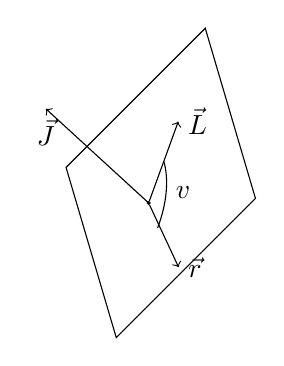
\begin{tikzpicture}[rotate around z=45, rotate around x=-45]
\draw (0,-0.3,0) -- (2.5,-0.3,0) -- (2.5,2.5,0) -- (0,2.5,0) -- cycle;
\draw[->] (1.,1.,0)node[draw,circle,inner sep=0] (o) {} -- (1.5,1.5,2)node[below] {$\vec{J}$};
\draw[->] (o) -- ++(295:0.9cm)node[right] {$\vec{r}$};
\draw[->] (o) -- ++(70:1.1cm)node[right] {$\vec{L}$}node [midway] (aux){};
\draw (aux) arc (0:-50:1) node[midway,right] {$v$};
\end{tikzpicture}

\label{fig:Lenztikz}

\end{figure}

\end{filecontents}%%contain tikz files as filecontents

\addtobeamertemplate{block begin}{\setlength\abovedisplayskip{2pt}\setlength\belowdisplayskip{2pt}\setlength\abovedisplayshortskip{2pt}\setlength\belowdisplayshortskip{2pt}}{}
\addtobeamertemplate{block begin}{\vspace*{-3pt}}{}
\addtobeamertemplate{block end}{}{\vspace*{-3pt}}

\begin{frame}
  \titlepage
\end{frame}

% Section and subsections will appear in the presentation overview
% and table of contents.
%\frame{\tableofcontents[onlyparts]}

\begin{frame}[label={argomenti}]{Fisica stellare: argomenti del corso}
\tableofcontents[onlyparts]
\end{frame}

\begin{wordonframe}{Perch\'e studio queste cose?? Sviluppi; futuro.}

Concretezza, concentrazione, indipendenza

\end{wordonframe}

\part{Intro}\label{part:intro}
\begin{wordonframe}{da fare: kippenhahn wiegert}
\begin{itemize}
\item strutture autogravitanti 1-62' (43)
\item metodi numerici 77'-84(44-48)
\item esistenza e unicit\'a 85'-99'(48-56)
\item Properties of stellar matter: ideal gas with radiation, ionization, degenerate electron gas, equazione di stato, opacit\'a 102'-144'(57-78)
\item produzione energia reazioni nucleari:  146'-172'(79-92)
\item politrope 174'-190' (93-102)
\item main sequence 207'-214' (110-114)
\item Hayashi line 224'-232' (119-123)
\item Stability 234'-246 (124-130)
\item Onset of star formation 248'-255' (131-134)
\item Formation of protostars 256'-265' (135-139)
\item pre-main sequence contraction 266'-270' (140-142)
\item from initial to present sun 271'-276' (142-144)
\item chemical evolution in MS 277'-291' (145-152)
\item He-burning: massive stars 292'-307' (153-160)
\item He-burning:low-mass stars 308'-327' (161-170)
\item Later phases:  328'-343' (171-178)
\item Explosion and collapse 344'-364' (179-189)
\end{itemize}
\end{wordonframe}
\section{Fonti}

\begin{wordonframe}{General}
Astrofisica stellare (castellani)
Rolfs rodney Couldron in the cosmos
iliadis nuclear burning
kippenhahn wiekert
salaris cassisi: evoluzione; popolazioni stellari;
\end{wordonframe}

\begin{wordonframe}{Milky way}
Thin disk thick disk transition
\end{wordonframe}

\begin{wordonframe}{popolazioni stellari}
salaris cassisi ch 9, 10, 11
\end{wordonframe}



\section{RegLez 19}\linkdest{reglez}
\begin{frame}[allowframebreaks]{Reg Lez 19}
\begin{itemize}
\phantomsection\linkdest{febbraio}
\item 18/02/2019 - Descrizione del corso. Descrizione generale della via Lattea. Definizione di ammasso stellare. Ammassi aperti ed ammassi globulari. Caratteristiche generali delle stelle di disco e di alone. Richiami alle definizioni di magnitudine, indice di colore, modulo di distanza. Cenni alla curva universale delle abbondanze (nel disco galattico). Alpha enhancement.  
\item 19/02/2019 - Caratteristiche generali del bulge e del thick disk. Discussione dell'origine dell'alpha enhancement. Scenario qualitativo generale della formazione della nostra Galassia. Alone interno ed alone esterno e relazione con la cattura di galassie nane durante la formazione della Galassia. Cenni alla formazione inside out del disco. Generalità su diagrammi colore- magnitudine di disco e di campo. Present day mass function ed initial mass function. Relazione massa-luminosit\'a. 
\item 22/02/2019 - Cenni alla derivazione dello Star formation rate e della relazione massa-luminosit\'a per il disco della nostra Galassia. Cenni alla produzione di elementi nella nucleosintesi primordiale. Generalit\'a sui metodi di determinazione delle abbondanze chimiche nel sistema solare. 
\item 25/02/2019 - Discussione del problema della determinazione dell'elio primordiale e dell'elio in stelle di disco. Cenni alla struttura del gruppo locale ed alle caratteristiche delle popolazioni stellari all'interno delle galassie del Gruppo Locale. Discussione del problema della multipopolazione negli ammassi globulari. 
\item 26/02/2019 - Generalit\'a su strutture autogravitanti. Stima del tempo scala dinamico. Richiamo al tempo di free fall. Equazioni di equilibrio stellare: equilibrio idrostatico ed equazione di continuit\'a. Peso molecolare medio. Esempio: calcolo del peso molecolare medio per materia completamente ionizzata. Peso molecolare medio degli ioni. Peso molecolare medio per elettrone. Generalit\'a sull'equazione del trasporto radiativo e sull'opacit\'a. Dimostrazione per ordini di grandezza che la presenza di un flusso negli interni stellari non contraddice l'assunzione di equilibrio termodinamico. 
\phantomsection\linkdest{marzo}
\item 01/03/2019 - Equilibrio termico per le stelle. Stima del tempo scala termico. Equazione dell'equilibrio termico (di conservazione dell'energia). Energia persa per neutrini; cenni ai processi principali. Calcolo della produzione di energia gravitazionale; problema della stima dell'energia gravitazionale del "primo modello" calcolato. 
\item 04/03/2019 - Integrazione delle equazioni di equilibrio stellare: interno, subatmosfera ed atmosfera. Cenni ai metodi di integrazione dell'atmosfera (variabile indipendente profondit\'a ottica). Metodo iterativo per il calcolo delle variabili fisiche esterne in atmosfera. Cenni al problema della determinazione della pressione di turbolenza e del gradiente ambientale nelle zone convettive esterne. Metodi numerici di integrazione delle equazioni di equilibrio stellare: il metodo del fitting. 
\item 05/03/2019 - Metodo di Henyey per l'integrazione delle equazioni di equilibrio stellare. Relazione tra energia termica ed energia gravitazionale in una struttura stellare all'equilibrio idrostatico. Il teorema del viriale per le strutture stellari: gas perfetto monoatomico e non monoatomico. Criterio di stabilit\'a per le strutture stellari in base al valore della costante adiabatica del gas. Relazioni per ordini di grandezza tra quantit\'a fisiche in strutture stellari ricavate utilizzando le equazioni di equilibrio stellare ed il teorema del viriale: relazione tra massa, densit\'a e temperatura, relazione tra luminosit\'a, massa, peso molecolare medio ed opacit\'a. 
\item 08/03/2019 - Approssimazione di strutture stellari a politropiche. Equazione di Lane-Emden e modalit\'a di risoluzione. Cenni a strutture isoterme. Esempio. il modello solare approssimato con una politropica. 
\item 11/03/2019 Equazione del trasporto radiativo. Generalit\'a sul trasporto di energia tramite conduzione elettronica. Coefficiente di diffusione per conduzione. Definizione dell'"opacità di conduzione" e sua stima approssimata nel gaso di gas degenere non relativistico. Generalit\'a su calcolo dell'opacit\'a radiativa. Calcolo dell'opacit\'a (in forma analitica) per: scattering elettronico, processi free free, fotoionizzazione. Opacit\'a nelle atmosfere stellari: opacit\'a di interazione fotoni-ione H- . 
\item 12/03/2019 - L'equazione di stato delle strutture stellari. Gas degenere elettronicamente. Effetti coulombiani nelle strutture stellari. Equazione di Saha.
\item  15/03/2019 - La media di Rosseland dell'opacità sulla distribuzione in frequenza dei fotoni. Discussione di grafici relativi all'andamento dell'opacit\'a negli interni stellari. Criterio di Schwarzschild per l'innesco della convezione. Cenni al problema dell'overshooting.
\item 18/03/2019 - Criterio di Ledoux per l'innesco della convezione nel caso di gas perfetto e non. Relazioni tra gradiente radiativo, ambientale ed adiabatico. Il gradiente ambientale negli interni e negli esterni stellari. Metodo della mixing length per il trattamento della convezione negli esterni stellari: Calcolo approssimato dell'altezza di scala della pressione, calcolo del flusso convettivo e del gradiente ambientale, in funzione della velocità media degli elementi di convezione.
\item 19/03/2019 - Teoria della mixing length per il calcolo del flusso convettivo: calcolo della velocità media degli elementi di convezione. Meccanismi di fusione nucleare nelle stelle. Sezione d'urto di fusione tra particelle cariche ed espressione per il rate di fusione nucleare. Picco di Gamow. Calcolo approssimato dei rates di fusione nucleare tra particelle cariche. Dipendenza approssimata delle reazioni nucleari tra particelle cariche dalla temperatura.
\item 22/03/2019 - Esempi di misure di sezioni d'urto nucleari. Sezione d'urto risonante: risonanze strette. Lo schermaggio elettronico in laboratorio. Calcolo approssimato dell'effetto di schermaggio elettronico in laboratorio. Lo schermaggio elettronico del plasma stellare: schermaggio debole e forte.
\item 25/03/2019 - Schermaggio elettronico nelle stelle. Calcolo dell'effetto di schermaggio debole. Correzione al rate di fusione dovuto alla presenza di schermaggio debole. Reazioni di fusione di elementi leggeri: deuterio, litio, berillio e boro. Fusione di idrogeno in elio: generalità e calcolo approssimato del flusso di neutrini solari. Reazione protone-protone: calcolo del tempo scala di fusione dei protoni nel Sole. Elementi primari ed elementi secondari in una catena di reazioni. Abbondanza di equilibrio degli elementi secondari. Esempio: calcolo dell' abbondanza di equilibrio del deuterio. Raggiungimento dell'abbondanza di equilibrio dell'elio 3 nella catena protone protone.
\item 26/03/2019 - Il bi-ciclo CN-NO: caratteristiche generali. Cenni allo spetto di neutrini solari. Cicli di CNO veloce. Dipendenza dalla temperatura della catena pp e del bi-ciclo CN-NO. Cenni alla caratteristiche delle stelle di sequenza principale inferiore e superiore dovute alle modalit\'a di combustione di H in He. Reazione 3 alfa per la fusione di elio in 12C e 12C+alfa per la produzione di 16 O. Confronto 12C + alfa e 16O + alfa alle condizioni fisiche tipiche della fusione di elio al centro.
\item 29/03/2019 - Influenza della sezione d'urto 12C + alfa sul tempo di vita in fase di combustione di elio centrale. Catene di produzioni di neutroni liberi. Reazioni in fasi evolutive avanzate: fusione di 12C, fotodisintegrazione del 20Ne, fusione dell'16O , fotosintegrazione del 28Si, catene di catture alfa su nuclei fino alla produzione di 56Fe.
\phantomsection\linkdest{aprile}
\item 01/04/2019 - Catture neutroniche su nuclei: andamento della sezione d'urto con l'energia e con il peso atomico. Processi s e processi r. Tempo di vita di un nucleo per cattura neutronica. Stima del flusso di neutroni caratteristico di processi s ed r. Stima dell'abbondanza di equilibrio per processi s. Spiegazione qualitativa dell'andamento dei picchi "s" ed "r" nella curva universale delle abbondanze. Cenni alle caratteristiche di protostella ed al passaggio tra protostella e stella di Pre-Sequenza Principale.
\item 02/04/2019 - Lezione seminariale del dott. Emanuele Tognelli su formazione stellare: tempo di Kelvin-Helmholtz, accrescimento della protostella fino al primo ed al secondo core idrostatico. Evoluzione di PMS: traccia di Hayashi.
\item 05/04/2019 - Lezione seminariale del dott. Tognelli su: evoluzione di Pre-Sequenza Principale. Ruolo dell'opacità dell'H- nella verticalit\'a della traccia di Hayashi, innesco della fusione del deuterio. Stelle completamente convettive. Stelle che in PMS sviluppano un nucleo radiativo.
\item 08/04/2019 - Zero Age Main Sequence. Approccio alla ZAMS per stelle di sequenza principale inferiore e superiore. Il profilo di abbondanza di equilibrio dell'3He. Caratteristiche generali delle stelle di sequenza principale inferiore e superiore. Dipendenza della posizione della ZAMS nel diagramma HR dall'abbondanza originale di elio e metalli. Accenno al metodo di determinazione di DY/DZ dal confronto teoria-osservazione per stelle di disco locale parallassate, Dipendenza della massa di transizione dall'abbondanza originale di elio e metalli. Massa minima e massima in ZAMS.
\item 09/04/2019 - Influenza sulla posizione della ZAMS del diagramma HR delle incertezze negli input fisici utilizzati dai modelli e nell'efficienza della convezione esterna. Metodo del Main Sequenze fitting per la determinazione della distanza di ammassi, criticit\'a del metodo. Evoluzione di sequenza principale per stelle di sequenza principale inferiore e superiore. Modalit\'a di esaurimento dell'H centrale per stelle di sequenza principale inferiore e superiore: Turn Off and Overall Contraction. Fase di subgigante rossa (SGB). Gap di Hertzsprung.
\item 12/04/2019 - Dalla fase di subgigante a quella di gigante rossa. Tracce evolutive ed isocrone di ammasso. Il Turn Off/Overall Contraction come indicatore di et\'a. Isocrone di ammassi giovani e vecchi. Evoluzione di gigante rossa: il primo dredge up.
\item 15/04/2019 - Morfologia del ramo delle giganti rosse per stelle di massa piccola ed intermedia: massa di "RGB transition". Dipendenza della massa di RGB transition dalla composizione chimica. Massa del nucleo di elio all'innesco dell'elio centrale in funzione della massa totale della stella. Luminosit\'a del vertice del ramo delle giganti rosse (RGB tip) in funzione della massa totale della stella. Dipendenza della massa del nucleo di elio all'innesco e della luminosità di RGB tip dalla composizione chimica. Dipendenza dell'isocrona e della luminosit\'a del TO/OC dall'abbondanza originale di elio e metalli. Influenza sull'isocrona e sulla luminosit\'a del TO della diffusione microscopica. Il bump dell'RGB. Dipendenza della luminosit\'a del bump dall'efficienza della convezione esterna, dall'et\'a dell'ammasso e dalla composizione chimica. Il tip dell'RGB come indicatore di distanza. Dipendenza della luminosit\'a del tip dalla composizione chimica. Innesco dell'elio a flash per stelle di piccola massa.
\item 16/04/2019 - Stelle in combustione centrale di elio: la ZAHB. Caratteristiche generali degli hot flashers. Il ramo orizzontale anomalo in ammassi stellari giovani a bassa metallicit\'a in galassie esterne: l'RGB clump. La Zero Age Horizontal Branch come indicatore di distanza. Dipendenza della luminosit\'a della ZAHB dalla composizione chimica. Cenni al metodo orizzontale per la determinazione dell'et\'a di ammassi antichi. Il metodo verticale per la determinazione dell'et\'a di ammassi antichi. Cenni alla discrepanza teoria-osservazione per la luminosit\'a del bump dell'RGB.
\item 29/04/2019 - Evoluzione in combustione di elio per stelle di ramo orizzontale. Combustione di elio centrale per stelle di massa intermedia; il clump dell'elio in ammassi di et\'a intermedia. Il clump dell'elio come indicatore di distanza. Combustione di elio centrale per stelle di massa intermedia-grande; il loop dell'elio. Incertezza nella determinazione di et\'a di ammassi antichi tramite il metodo verticale.
\item 30/04/2019 - Effetto dell'overshooting sui modelli di sequenza principale superiore e sulla determinazione di et\'a di ammassi di et\'a giovane-intermedia. Incertezze sulla determinazione di et\'a di ammassi di et\'a giovane-intermedia. Discussione sui parametri che influenzano la morfologia di ramo orizzontale.
\phantomsection\linkdest{maggio}
\item 03/05/2019 - Effetto della presenza di diffusione microscopica sulla determinazione dell'et\'a tramite il metodo verticale. Il parametro R per la determinazione dell'elio. Esaurimento dell'elio centrale: autotrascinamento del nucleo, semiconvezione e pulsi convettivi.
\item 06/05/2019 - Ingresso in fase di ramo asintotico: il clump dell'AGB. AGB manque'. Evoluzione di ramo asintotico: il secondo dredge-up. Pulsi termici e terzo dredge-up. Nucleosintesi di elementi s in AGB: la tasca di 13C. Produzione di litio in AGB.

\item 07/05/2019 - Lezione seminariale del dott. Emanuele Tognelli su: abbondanza superficiale di elementi leggeri in fase di Pre-Sequenza Principale. Il metodo del "lithium depletion boundary" per la datazione di ammassi giovani.
\item 10/05/2019 - Caratteristiche generali dell'evoluzione avanzata di stelle massicce. Destino finale di stelle di varia massa: nane bianche di He, C/O, O/Ne, supernovae di tipo II da deflagrazione del carbonio e da cattura elettronica su nuclei, supernovae di tipo II da fotodisintegrazione del ferro.
\item 13/05/2019 - lezione: Discussione sul 60Fe come elemento indicatore di esplosioni di supernova nelle vicinanze della Terra negli ultimi milioni di anni. Supernovae di tipo II: caratteristiche di pre-supernova. Emissione di neutrini e loro interazione con i nuclei del nocciolo denso della supernova. Intrappolamentp e temposcala di emissione dei neutrini. Stima per ordini di grandezza dell'energia emessa sotto varie forme (neutrini, fotoni, energia del fronte di shock). Neutronizzazione esplosiva e meccanismo di esplosione ritardata. Discussione sulle caratteristiche della supernova 1987A, sul flusso di neutrino osservato e sulla sua osservazione in varie bande elettromagnetiche nelle varie fasi di supernova.. Classificazione dei vari tipi di supernovae in base allo spettro ed alla morfologia della curva di luce.
\item 14/05/2019 - Lezione seminariale del prof. Prada Moroni su evoluzione delle nane bianche.
\item 17/05/2019 - Caratteristiche e metodo di calcolo del modello solare standard. Generalita' sull'eliosismologia e sui modelli solari eliosismologici. Generalità sulla rivelazione dei neutrini solari come test aggiuntivo del modello solare standard.
\item 20/05/2019 - Stelle variabili pulsanti: cenni al meccanismo di pulsazione. La striscia di instabilita' nel diagramma HR ed i vati tipi di stelle variabili pulsanti. RR Lyrae: diagramma di Bailey, curve di luce, relazione periodo, luminosita', massa e temperatura effettiva. Le RR Lyrae come indicatori di distanza. Il parametro A come indicatore di elio. Stelle cefeidi classiche. Uso delle stelle cefeidi come indicatori di distanza di ammasso e di campo. La dicotomia di Oosterhoff.
\item 21/05/2019 - Lezione seminariale del dott. Cignoni su studi di popolazione nella galassie esterne: recupero della star formation history. Analisi di popolazioni non risolte semplici e complesse.
\item 24/05/2019 - lezione: Caratteristiche generali delle SNIa. Possibili progenitori della SNIa: generalità su meccanismi di scambio di massa in sistemi binari, sistemi finali dopo due common envelope, possibili scenari di accrescimento di H/He/C su una compagna degenere. La SNIa come indicatori di distanza.
\end{itemize}
\end{frame}

\section{RegLez 17}

\begin{frame}[allowframebreaks]{Reg Lez 17}
\begin{itemize}
\item testo: Popolazioni stellari: formazione stellare (fenomenologia)
\item lezione: Descrizione generale della struttura della nostra Galassia. Concetti base: parallasse, magnitudine assoluta ed apparente, modulo di distanza, estinzione ed arrossamento. Caratteristiche generali di ammassi aperti e globulari. Alpha enhancement.
\item lezione: Caratteristiche fotometriche, dinamiche e chimiche delle popolazioni stellari della nostra Galassia. Caratteristiche generali delle stelle di thick disk. Relazione massa-luminosit\'a per le stelle di sequenza principale. Relazione generale tra massa e tempo di vita di una stella. Initial Mass Function and Present Day Mass Function.
\item lezione: Differenze generali tra stelle di ammasso e stelle di campo. Esempi di diagrammi Colore-Magnitudine di stelle di ammasso e stelle di campo. Discussione generale sullo studio delle caratetristiche delle stelle di campo. Cenni alla determinazione dello ''Star Formation Rate'' per il disco della nostra Galassia ed alla determinazione della relazione et\'a-metallicit\'a. 
\item lezione: Scenario generale di formazione della Via Lattea. Cenni alle galassie del Gruppo Locale. Cenni alle popolazioni stellari nella Via Lattea e nella galassie del Gruppo Locale. Metodi di determinazione delle abbondanze stellari. La curva ''universale'' delle abbondanze. Cenni alla nucleosintesi primordiale.
\item lezione: Discussione generale sulla multipopolazione negli ammassi globulari della nostra Galassia. 
\item Testo: Equazioni struttura stellare: fenomenologia e metodi numerici
\item lezione: Equilibrio idrostatico nelle stelle. Equazioni di equilibrio stellare: equilibrio idrostatico ed equazione di continuit\'a.
\item lezione: Peso molecolare medio. Esempio: calcolo del peso molecolare medio per materia completamente ionizzata. Peso molecolare medio degli ioni. Peso molecolare medio per elettrone. Generalit\'a sull'equazione del trasporto radiativo. Equilibrio termico. Le equazioni di equilibrio stellare. Calcolo dell'energia "gravitazionale".
\item lezione: Calcolo approssimato del tempo scala termico nell'interno del Sole. L'equazione del trasporto nelle atmosfere stellari. Profondit\'a ottica. Equazioni di equilibrio stellare in atmosfera. Generalit\'a sui metodi numerici di integrazione delle equazioni di equilibrio stellare. Il metodo del fitting.
\item lezione: Seminario del dott. Tognelli su: l'equazione di stato delle strutture stellari. Gas degenere elettronicamente. Effetti coulombiani nelle strutture stellari. Equazione di Saha.
\item lezione: Il metodo di Henyey per la risoluzione delle equazioni di equilibrio stellare. Integrazione dell'atmosfera. L'equazione del trasposto radiativo. Il teorema del viriale per le strutture stellari: caso di gas perfetto monoatomico. Tempo scala di Kelvin-Helmholtz.
\item lezione: Il teorema del viriale: gas perfetto non monoatomico. Criterio di stabilit\'a delle strutture stellari. Utilizzo delle equazioni di equilibrio stellare e del teorema del viriale per ottenere relazioni per ordini di grandezza tra: 1) massa, densit\'a e temperatura delle stelle 2) massa-luminosit\'a.
\item lezione: Calcolo approssimato dell'opacit\'a da scattering Thompson nel caso di ionizzazione totale. Formula di Kramer per opacit\'a free-free e bound free. Opacit\'a legata agli ioni H-.
\item lezione: La conduzione elettronica. Opacit\'a conduttiva. Equazione del trasporto in presenza di opacit\'a conduttiva. Criterio di Schwarzschild e di Ledoux per l'innesco della convezione in ambiente stellare. Cenni al fenomeno dell'overshooting.
\item lezione: Il metodo della mixing lenght per il trattamento della convezione negli inviluppi esterni stellari. Calcolo approssimato dell'altezza di scala della pressione. 
\item lezione: La teoria della mixing lenght per il trattamento della convezione negli esterni stellari: calcolo del flusso convettivo, della velocit\'a media delle bolle di convezione e del gradiente ambientale negli esterni stellari. Modelli politropici di strutture stellari: equazione di Lane-Emden e calcolo dell'andamento di pressione e densit\'a per modelli stellari politropici. Esempi: il modello solare.
\item Testo: Produzione enrgia: reazioni nucleari (evoluzione)
\item lezione: Calcolo dei rates di reazioni di fusione nucleare tra particelle cariche. La probabilit\'a di penetrazione della barriera coulombiana ed il fattore astrofisico. Il picco di Gamow. Espressione approssimata dei rates di fusione nucleare. Dipendenza approssimata delle reazioni dalla temperatura.
\item lezione: Lo schermaggio elettronico in laboratorio. Lo schermaggio elettronico nel plasma stellare: schermaggio debole, intermedio e forte. Trattamento dello schermaggio debole negli interni stellari secondo il metodo di Salpeter. 
\item lezione: Reazioni nucleari di combustione di elementi leggeri. Elementi primari ed elementi secondari. Concentrazione di equilibrio per gli elementi secondari. Reazioni di fusione di H in He: la catena protone-protone ed il bi-clo CN-NO. Neutrini solari.
\item lezione: Reazioni del ciclo CNO veloce. Reazioni di fusione di elio in C ed O. Catene di produzione di neutrini liberi in fasi evolutive avanzate.
\item lezione: Reazioni di fusione del C e dell'O. Reazioni nucleari successive fino alla produzione degli elementi del picco del ferro. Struttura a cipolla di pre-supernova e nucleosintesi esplosiva. Catture neutroniche su nuclei: processi s e processi r. Sezione d'urto per cattura neutronica ed andamento con l'energia del rate delle reazioni di cattura neutronica. Stima del flusso di neutroni caratteristico di processi s ed r. Stima dell'abbondanza di equilibrio per processi s. Spiegazione qualitativa dell'andamento dei picchi "s" ed "r" nella curva universale delle abbondanze.
\item Testo: MS-PMS
\item lezione: Seminario del dott. Emanuele Tognelli su caratteristiche delle fasi di protostella e di Pre-Sequenza Principale (PMS). Traccia di Hayashi. Effetto di variazione di massa e composizione chimica in PMS. Combustione del deuterio ed effetti sulle strutture di PMS.
\item lezione: Caratteristiche e metodo di calcolo del solare standard. Generalit\'a sull'eliosismologia e sui modelli solari eliosismologici.
\item lezione: Seminario del dott. Tognelli su evoluzione di Pre-sequenza principale, evoluzione temporale dell'abbondanza superficiale di elementi leggeri. Ingresso in ZAMS per stelle di sequenza principale inferiore e superiore.
\item lezione: Dipendenza della posizione di PMS nel diagramma HR dalla composizione chimica e dall'efficienza della convezione esterna. Zero Age Main Sequence. Dipendenza della posizione di ZAMS nel diagramma HR dalla composizione chimica e dall'efficienza della convezione esterna. Stelle di sequenza principale inferiore e superiore. Approccio alla ZAMS: sviluppo di un piccolo nucleo convettivo per stelle di SPI durante il raggiungimento dell'abbondanza di equilibrio dell'3He. Profilo dell'abbondanza di equilibrio dell'3He per stelle di SPI.Very low mass. Calcolo approssimativo della massa minima per l'innesco della fusione di H in He. 
\item lezione: Evoluzione di sequenza principale. Modalit\'a di esaurimento dell'idrogeno centrale per stelle di sequenza principale inferiore e superiore. Fase di subgigante rossa. Isocrona di ammasso. La luminosit\'a all'esaurimento dell'idrogeno centrale come indicatore di et\'a di una popolazioen stellare semplice. 
\item lezione: Incertezze nelle previsioni teoriche di MS. Generalit\'a sulle isocrone di ammasso. Il metodo del fitting della MS per la determinazione della disatnza degli ammassi globulari. La luminosit\'a del TO/OC come indicatore di et\'a. Evoluzione di sub-gigante rossa. Dipendenza delle tracce di MS/SGB dalla composizione chimica. Influenza della diffusione sulla traccia di stelle di data massa nel diagramma HR.
\item Testo: Post Hydrogen
\item lezione: Evoluzione di gigante rossa: il primo dredge up ed il bump dell'RGB. Dipendenza della luminosit\'a del bump dalla composizione chimica. Perdite di massa in RGB. Il flash dell'elio. Morfologia dell'RGB per ammassi stellari giovani ed antichi.
\item lezione: Massa dell'elio all'innesco dell'elio centrale in funzione della massa totale della stella. Massa di RGB transition e sua dipendenza dalla composizione chimica. Dipendenza della luminosit\'a del vertice del ramo della giganti rosse dalla composizione chimica. Il tip dell'RGB come indicatore di distanza.
\item lezione: Dipendenza dell'isocrona dalla composizione chimica e dalla diffusione. Fase di combustione di elio per stelle di ammasso antico: il ramo orizzontale, HB. Zero Age Horizontal Branch. Il ramo orizzontale come candela campione, metodo verticale per la determinazione dell'et\'a di ammassi antichi. Dipendenza della ZAHB dalla composizione chimica.
\item lezione: Influenza della diffusione sulla determinazione dell'et\'a degli ammassi tramite il metodo verticale. Evoluzione di ramo orizzontale. Morfologia del ramo orizzontale: dipendenza da metallicit\'a ed et\'a dell'ammasso. Hot flashers. Il clump dell'elio ed il loop dell'elio. Il clump dell'elio come indicatore di distanza.
\item lezione: Effetto della presenza di overshooting sulla determinazione di et\'a di ammassi giovani. Discussione dell'incertezza sulla detrminazione di et\'a in ammassi stellari. Evoluzione in combustione di elio centrale: autotrascinamento e semiconvezione. Il parametro R per la stima dell'abbondanza di elio in ammassi antichi.
\item lezione: Cenni su stelle variabili come indicatori di distanza: RR Lyrae e cefeidi classiche. Ingresso in ramo asintotico. Il clump dell'AGB in stelle di piccola massa. Caratteristiche generali per stelle di AGB. Il secondo dredge up. Nucleosintesi in AGB. Pulsi termici.
\item lezione: Evoluzione della luminosit\'a durante i pulsi termici. Terzo dredge up, hot bottom burning. Catene di produzione di neutroni liberi e processi s in fase di ramo asintotico.
\item lezione: Evoluzione finale di stelle di varia massa. Nane bianche di C/O e O/Ne, supernovae di tipo II da deflagrazione del carbonio e da cattura elettronica su nuclei. Supernovae di tipo II da fotodisintegrazioen del ferro.
\item Lezione seminariale del prof. Prada Moroni su caratteristiche strutturali delle nane bianche, curva di raffreddamento di nana bianca. Misura di distanza ed et\'a in ammasso tramite la curva di raffreddamento delle nane bianche.
\item lezione: Lezione seminariale del prof. Cignoni su popolazioni stellari complesse nelle vicinanze del Sole e nelle galassie nane. recupero della star formation rate in popolazioni complesse.
\end{itemize}
\end{frame}

\part{Stellar population in the milky way}\label{part:gaxpops}
\begin{frame}{this part toc}
\begin{itemize}
\item Solar neighborhood
\end{itemize}
\end{frame}

\part{Equazioni struttura stellare}\label{part:starstruct}

\begin{frame}{this part toc}
\begin{itemize}
\item Tempi scala
\end{itemize}
\end{frame}

\part{Reazioni nucleari}\label{part:reactions}

\begin{frame}{this part toc}
\begin{itemize}
\item Tempi scala
\end{itemize}
\end{frame}

\part{Evoluzione stellare}\label{part:evolphs}

\begin{frame}{this part toc}
\begin{itemize}
\item Tempi scala
\end{itemize}
\end{frame}


\end{document}